\chapter{Materiał i metoda badawcza}

W ramach pracy przeprowadzone zostały badania dotyczące klasyfikacji choroby Parkinsona.
Głównym celem było opracowanie efektywnego modelu klasyfikacji binarnej, który może rozróżniać
osoby z PD od osób zdrowych na podstawie analizy sygnałów mowy.
Przyjęte podejście opiera się na wykorzystaniu metod przetwarzania sygnałów mowy oraz
uczenia maszynowego. Najpierw zebrano dane, w tym nagrania głosowe osób z chorobą Parkinsona
(PD) oraz osób zdrowych (HC, ang. \emph{Healthy Controls}). Następnie przeprowadzono analizę przy użyciu różnych ustawień
spektrogramów i melspektrogramów. Obejmuje to zmienne parametry takie jak rozmiar okna i
przesunięcie okna. Dodatkowo, przeprowadzono badania dotyczące różnych architektur
konwolucyjnych sieci neuronowych. Celem jest zbadanie, które architektury sieci i ustawienia
spektrogramów dają najlepsze wyniki w klasyfikacji choroby Parkinsona dla poszczególnych
samogłosek. Przeprowadzona analiza porównawcza pozwala na lepsze zrozumienie wpływu tych
czynników na skuteczność klasyfikacji. W rezultacie, możliwe będzie ustalenie optymalnych ustawień i
architektur dla klasyfikacji choroby Parkinsona na podstawie analizy sygnałów mowy. Ponadto zbadano
wpływ rozszerzenia zbioru danych o dodatkowe nagrania pochodzące od tych samych osób.

\begin{figure}[htbp]
	\centering
	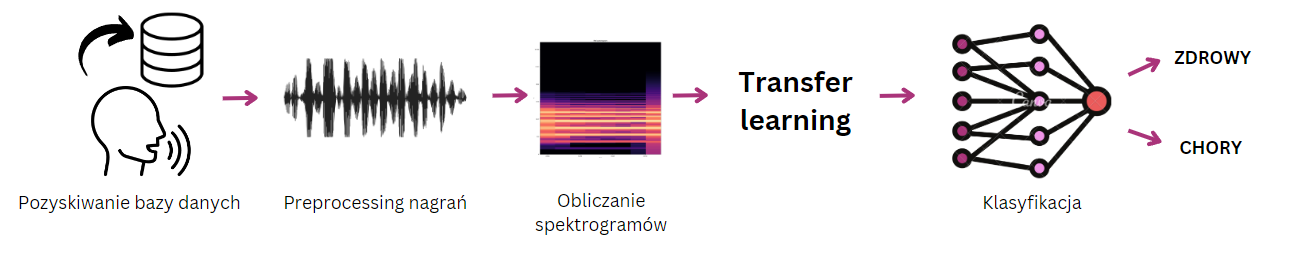
\includegraphics[width=1\textwidth]{./img/methodology}
	\caption{Schemat przyjętej metody badawczej}
    \label{fig:methodology}
\end{figure}

%---------------------------------------------------------------------------

\section{Materiał badawczy}
\label{sec:material-badawczy}

Materiałem badawczym w niniejszej pracy magisterskiej są nagrania głosowe podtrzymywanych samogłosek (ang. \emph{sustained vowels}) /a/, /e/, /i/, /o/ oraz /u/, ze względu na największą uniwersalność.
Baza danych obejmuje nagrania osób zdrowych oraz z chorobą Parkinsona.
Podstawą skuteczności metod uczenia maszynowego jest odpowiednie przygotowanie danych, zarówno pod względem jakości, jak i ilości.
To kluczowy element, który wpływa na wydajność i zdolność modelu do radzenia sobie w rzeczywistym środowisku.
Dane użyte do trenowania modelu muszą być dokładne, spójne i reprezentatywne dla rzeczywistego środowiska, w którym będzie działał model.

Dlatego model uczenia maszynowego musi być trenowany na wystarczająco dużej ilości danych.
Jest to podobne do procesu nauki lekarza – im więcej przypadków lekarz widzi i diagnozuje, tym lepiej radzi sobie z różnymi przypadkami w praktyce.
W  uczeniu maszynowym większa ilość danych pozwala na uchwycenie różnic międzyosobniczych i niuansów w danych, co przekłada się na większą stabilność i skuteczność modelu.
Model musi być w stanie radzić sobie z nowymi danymi, które nie były używane podczas treningu.

W badaniu opublikowanym w artykule~\cite{SustainedVowelsProblems} podkreślono, że często osoby zajmujące się rozwiązaniami do automatycznej diagnozy choroby Parkinsona na podstawie mowy polegają na jednym konkretnym zbiorze danych.
Takie podejście może prowadzić do wyników, które są zbyt optymistyczne, ze względu na różnice związane z językiem ojczystym osób badanych oraz warunki i sposób przeprowadzania nagrań.

Biorąc pod uwagę powyższe, podjęto decyzję o połączeniu trzech różnych baz danych w językach polskim, włoskim oraz hiszpańskim.
Ta inicjatywa badawcza ma na celu zbadanie potencjalnej uniwersalności narzędzia służącego do automatycznej diagnozy choroby Parkinsona, tak by nie było ograniczone tylko do jednej grupy narodowościowej.
Ponadto można by uniknąć potencjalnych błędów wynikających z języka ojczystego osób badanych czy lokalnych warunków nagrywania.
Pozwoliłoby to na rozwinięcie bardziej ogólnego i zastosowalnego narzędzia diagnostycznego, które może być używane na skalę międzynarodową, przyczyniając się do poprawy jakości opieki zdrowotnej i diagnozy tej choroby.

Ponadto żaden z dostępnych publicznie korpusów nie zawiera wystarczającej ilości nagrań by mówić o stabilnym rozwiązaniu.
Łączenie korpusów może znacząco poprawić zdolności generalizacyjne modelu.

\subsection{Baza danych w języku polskim}
\label{subsec:polska-baza}

Materiał badawczy pochodzący od osób cierpiących na chorobę Parkinsona (PD) i posługujących się językiem polskim, został zgromadzony podczas
realizacji rozprawy doktorskiej we współpracy z Krakowskim Szpitalem Specjalistycznym im.
Jana Pawła II~\cite{daria:2018}.
Zawarta w bazie danych kolekcja obejmuje nagrania samogłosek /a/, /e/, /i/, /o/ oraz /u/ z wydłużoną intonacją, pozyskane od 27 pacjentów.
Dla każdego z pacjentów dostępne jest jedno nagranie każdej z wymienionych samogłosek.
W ramach przeprowadzonych badań pomiary zostały wykonane przed spożyciem leków oraz w określonych odstępach czasowych po podaniu lewodopy.
Przed każdym pomiarem lekarz neurolog przeprowadzał badanie pacjenta i oceniał jego stan, wykorzystując skalę UPDRS\@.
W niniejszej pracy magisterskiej wykorzystano jedynie nagrania głosowe zarejestrowane przed podaniem leku.

Nagrania osób zdrowych zostały zebrane w ramach pracy przy wykorzystaniu aplikacji \emph{Easy Voice Recorder}, która jest programem do nagrywania dźwięku.
Ustalono protokół nagrywania, wykluczając osoby poniżej 50 roku życia, palące oraz ze zdiagnozowaną lub podejrzewaną chorobą wpływającą na aparat mowy lub korę mózgową (np. choroba Parkinsona, epilepsja, padaczka).
Pozyskiwano nagrania jedynie od osób, dla których językiem ojczystym jest polski.
W tabeli~\ref{tab:polish_database} przedstawiono informacje dotyczące bazy danych.

\begin{table}[h]
\centering
\caption{Charakterystyka polskiej bazy danych}
\label{tab:polish_database}
\begin{tabular}{|l|c|c|c|}
\hline
\textbf{Kategoria} &\textbf{Osoby zdrowe (HC)} &\textbf{Osoby chore (PD)} &\textbf{Razem} \\ \hline
Liczba osób &26 &27 &53\\ \hline
Liczba nagrań &67 &27 &94\\ \hline
Średnia wieku &60,88 ± 7,98 &64,49 ± 8,49  &62,68 ± 8,43\\ \hline
Liczba kobiet &18 &13 &31\\ \hline
Liczba mężczyzn &8 &14 &22 \\ \hline
\end{tabular}
\end{table}

Każda osoba kwalifikująca się do badania otrzymała zadanie trzykrotnego wypowiedzenia
samogłosek /a/, /e/, /i/, /o/ oraz /u/ w odstępach czasowych, utrzymując dźwięk przez co najmniej 2 sekundy.
Następnie nagrania zostały dokładnie przeanalizowane.
Usunięto nagrania zbyt krótkie oraz te, które nie spełniały kryteriów dotyczących jakości.
Otrzymana baza danych nadal zawierała nagrania od 27 osób chorych oraz od 26 osób zdrowych, zmieniła się jedynie liczebność nagrań dla poszczególnych
samogłosek.

\subsection{Baza danych w języku włoskim}
\label{subsec:wloska-baza}

Włoska baza danych to \emph{Italian Parkinson's Voice And Speech} dostępna na platformie \emph{IEEEDataPort}.
Dane zostały zebrane na cele artykułu~\cite{italian-database}, który badał zrozumiałość mowy w chorobie Parkinsona z wykorzystaniem systemu \emph{speech-to-text}.
Zbiór zawiera wiele różnych podzbiorów, ale wykorzystano jedynie podtrzymywane samogłoski /a/, /e/, /i/, /o/ oraz /u/.
Ocena stopnia zaawansowania choroby została przeprowadzona przy pomocy skali UPDRS.
Wszystkie nagrania pochodzą od osób, dla których natywnym językiem jest włoski.
Początkowo baza danych zawiera nagrania od 50 osób, jednak po wstępnym oczyszczeniu wykorzystano jedynie 45. Charakterystykę zbioru przedstawiono w tabeli~\ref{tab:italian-database}

\begin{table}[h]
\centering
\caption{Charakterystyka włoskiej bazy danych}
\label{tab:italian-database}
\begin{tabular}{|l|c|c|c|}
\hline
\textbf{Kategoria} &\textbf{Osoby zdrowe (HC)} &\textbf{Osoby chore (PD)} &\textbf{Razem} \\ \hline
Liczba osób &19 &26 &45\\ \hline
Liczba nagrań &38 &52 &90\\ \hline
Średnia wieku &67,31 ± 5,23 &66,96 ± 8,59  & 67,11 ± 7,36 \\ \hline
Liczba kobiet &10 &7 &17\\ \hline
Liczba mężczyzn &9 &19 &28 \\ \hline
\end{tabular}
\end{table}


\subsection{Baza danych w języku hiszpańskim}
\label{subsec:hiszpanska-baza}


Hiszpańska baza danych nazywana jest PC-GITA i została zaprezentowana w publikacji~\cite{pc-gita}.
Zawiera nagrania mowy 50 pacjentów z PD i ich tyle samo osób zdrowych, dopasowanych pod względem wieku i płci.
Wszyscy uczestnicy są hiszpańskojęzycznymi native speakerami, a nagrania zostały zebrane zgodnie z protokołem uwzględniającym wymagania
techniczne oraz kilka zaleceń ekspertów z dziedzin lingwistyki, foniatryki i neurologii.
Kolekcja obejmuje takie zadania jak trwałe wymawianie samogłosek, ocenę dyadokokinetyczną, 45 słów, 10 zdań, tekst do czytania i monolog.
Podobnie jak w przypadku pozostałych baz wykorzystano jedynie nagrania samogłosek /a/, /e/, /i/, /o/ oraz /u/.
Szczegółowa charakterystyka zbioru została przedstawiona w tabeli~\ref{tab:spanish-database}

\begin{table}[h]
\centering
\caption{Charakterystyka hiszpańskiej bazy danych}
\label{tab:spanish-database}
\begin{tabular}{|l|c|c|c|}
\hline
\textbf{Kategoria} &\textbf{Osoby zdrowe (HC)} &\textbf{Osoby chore (PD)} &\textbf{Razem} \\ \hline
Liczba osób &50 &50 &100\\ \hline
Liczba nagrań &150 &150 &300\\ \hline
Średnia wieku &60,90 ± 9,37 &61,14 ± 9,51  &61,02 ± 9,15\\ \hline
Liczba kobiet &25 &25 &50\\ \hline
Liczba mężczyzn &25 &25 &50 \\ \hline
\end{tabular}
\end{table}

\subsection{Podsumowanie wykorzystanych baz danych}
\label{subsec:podsumowanie-baz}

Połączenie baz danych było możliwe ze względu na uniwersalność podstawy diagnostycznej jakiej są podtrzymywane samogłoski.
Nagrania różniły się długością, jednak wykorzystano jedynie krótkie fragmenty, więc nie stanowiło to problemu.
Wszystkie zostały zarejestrowane z częstotliwością próbkowania 44,1 kHz.

Trudno nie zauważyć znaczącej przewagi liczby nagrań w bazie hiszpańskojęzycznej (Rys.~\ref{fig:language-distribution}).
Jednak zdecydowano się na rezygnację z wyrównywania liczby nagrań w poszczególnych językach, z uwagi na to, że baza danych jest już stosunkowo niewielka, i dodatkowe ograniczenie liczby nagrań mogłoby znacząco zmniejszyć jej wartość i możliwości badawcze.

Zachowano zbliżone proporcje wieku (różnica w średniej wieku mniejsza niż 5 lat) i płci pomiędzy grupą pacjentów a grupą porównawczą.
Drobne różnice w liczbie próbek w poszczególnych przedziałach wiekowych nie powinny mieć istotnego wpływu na wyniki klasyfikacji.
Szczegółowe charakterystyki zbioru danych zostały przedstawiona na Rys.~\ref{fig:age-distribution} i~\ref{fig:gender-distribution}.


\begin{figure}
    \begin{subfigure}{0.9\textwidth}
        \centering
       	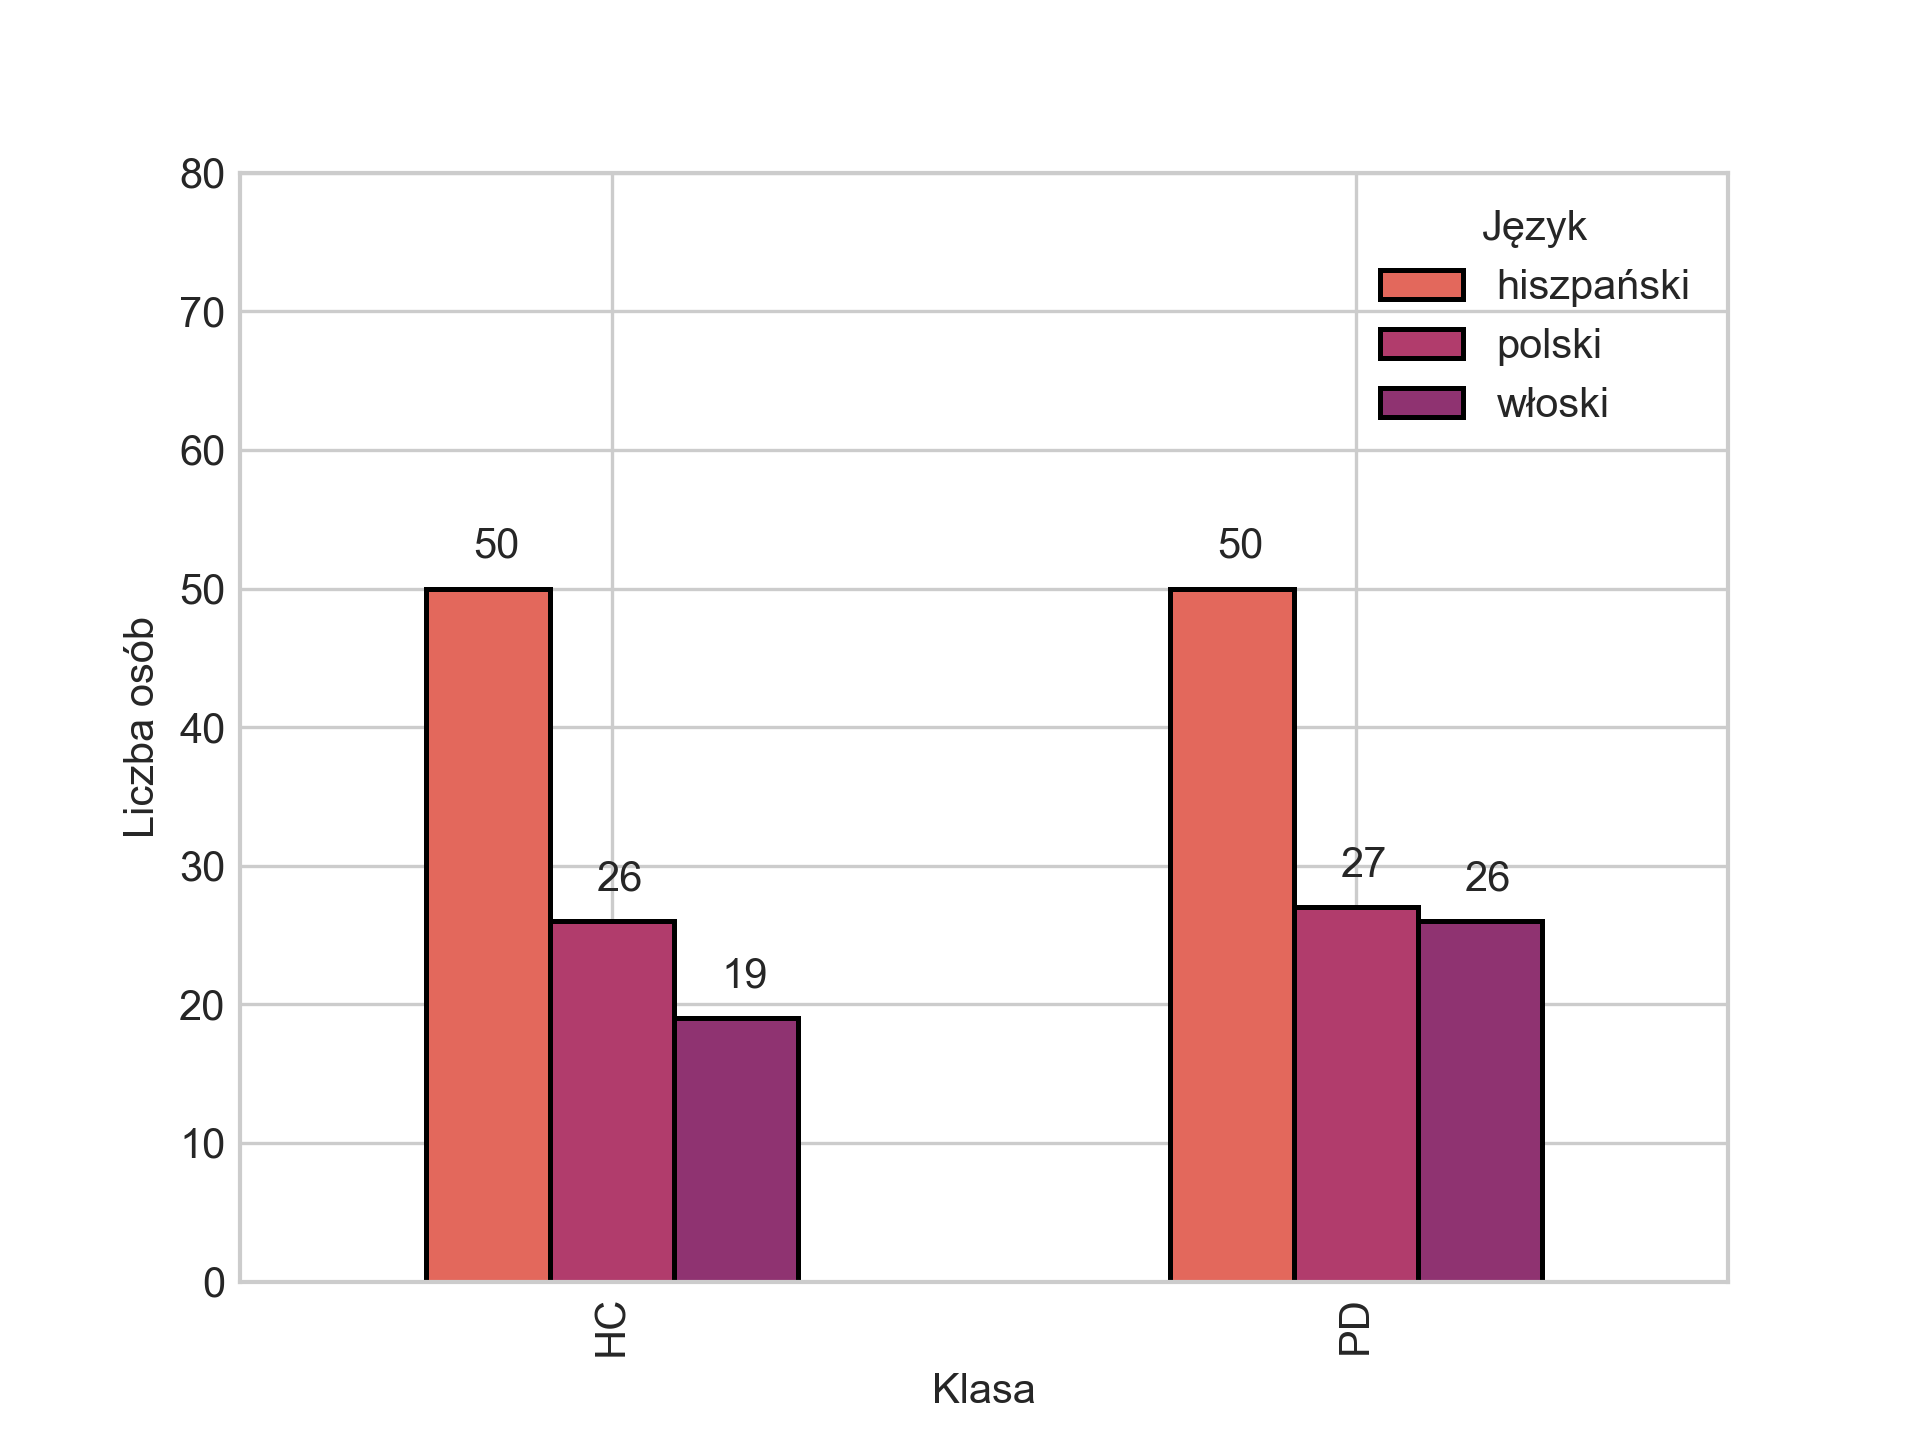
\includegraphics[width=0.60\textwidth]{./img/database stats/languages_distribution}
	    \caption{Udział nagrań w poszczególnych językach w ostatecznej bazie danych}
        \label{fig:language-distribution}
    \end{subfigure}

    \begin{subfigure}{0.9\textwidth}
        \centering
        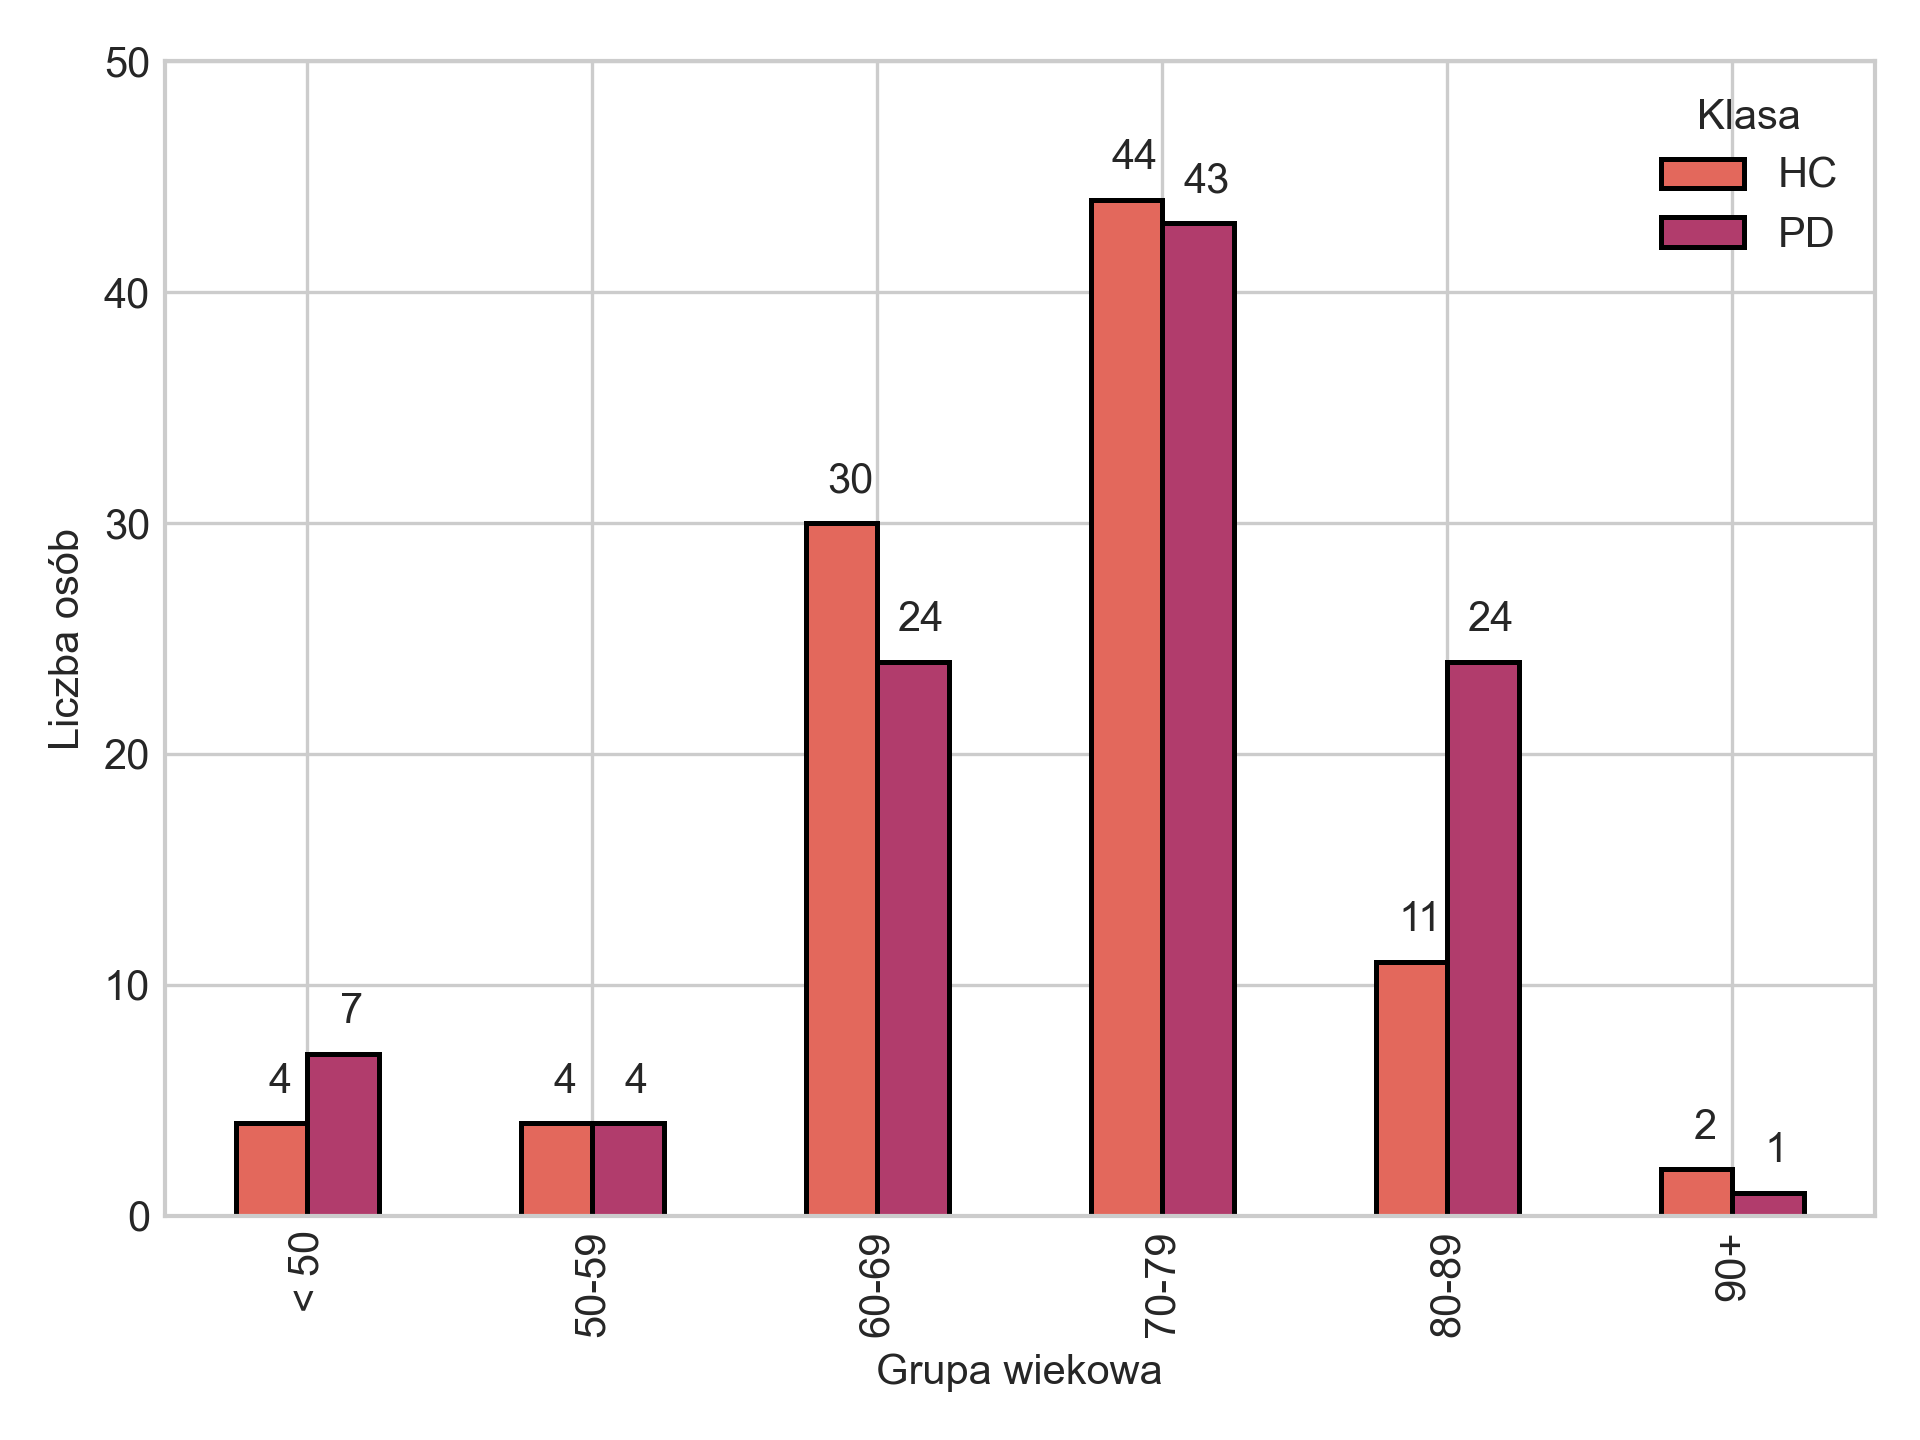
\includegraphics[width=0.60\textwidth]{./img/database stats/age_distribution}
        \caption{Rozkład klas w grupach wiekowych}
        \label{fig:age-distribution}
    \end{subfigure}

    \begin{subfigure}{0.9\textwidth}
        \centering
       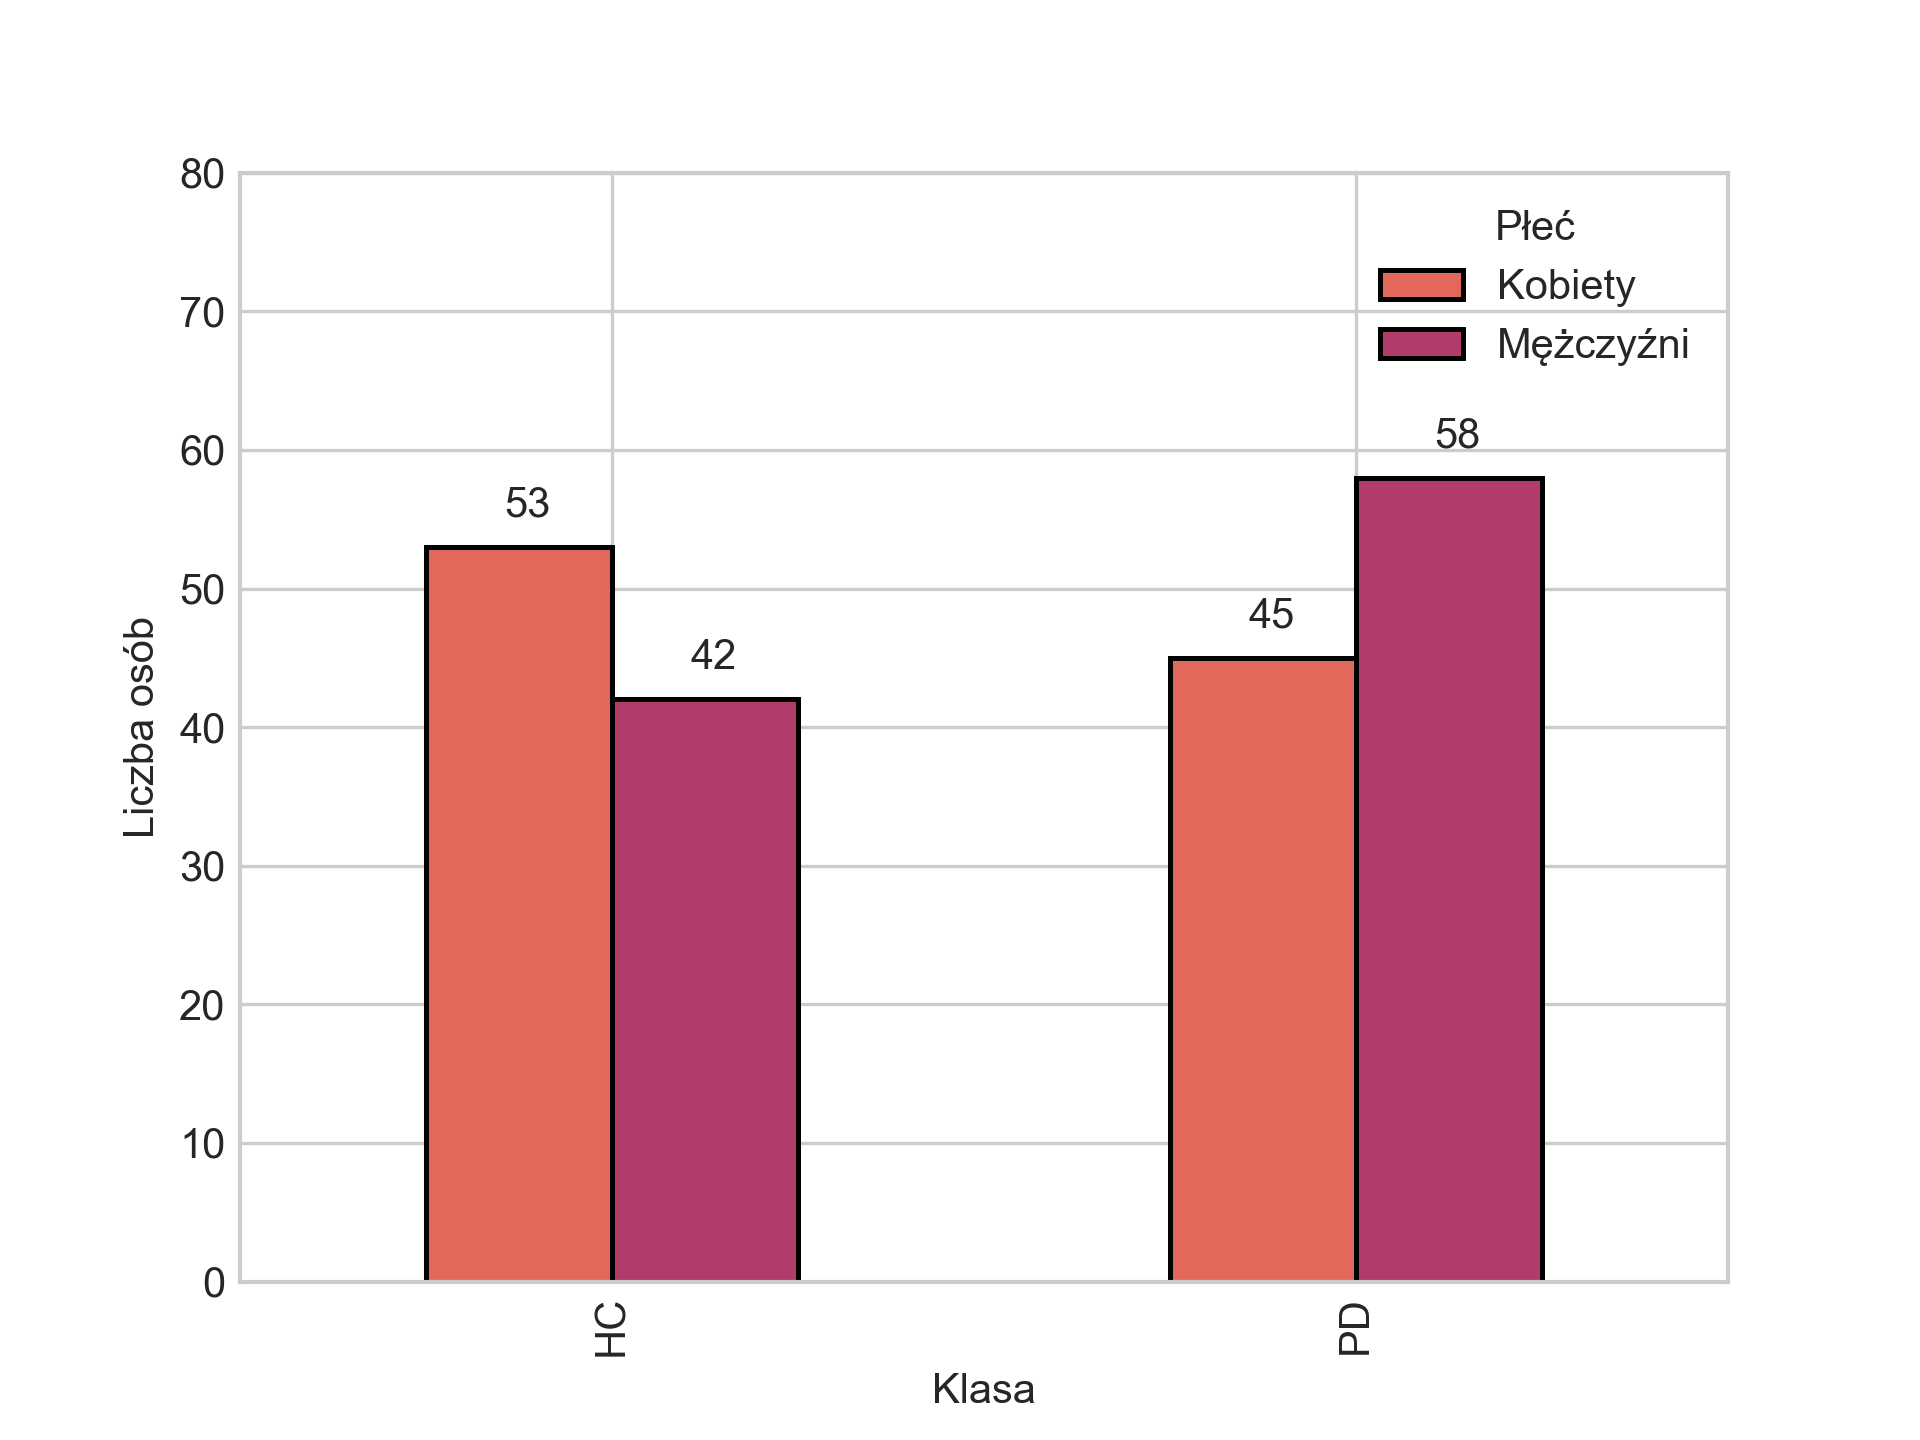
\includegraphics[width=0.65\textwidth]{./img/database stats/gender_distribution}
	    \caption{Rozkład płci w klasach}
        \label{fig:gender-distribution}
    \end{subfigure}

    \caption{Charakterystyka wykorzystanej bazy danych}
    \label{fig:charakterystyka-bazy}
\end{figure}



\begin{table}[h]
\centering
\caption{Charakterystyka stworzonej bazy danych}
\label{tab:summary-database}
\begin{tabular}{|l|c|c|c|}
\hline
\textbf{Kategoria} &\textbf{Osoby zdrowe (HC)} &\textbf{Osoby chore (PD)} &\textbf{Razem} \\ \hline
Liczba osób &95 &103 &198\\ \hline
Liczba nagrań &255 &229 &484\\ \hline
Średnia wieku & 62,18 ± 8,70 & 62,84 ± 9,45  & 62,32 ± 8,99 \\ \hline
Liczba kobiet &53 &45 &98\\ \hline
Liczba mężczyzn &42 &58 &100 \\ \hline
\end{tabular}
\end{table}

%Jednym z głównych celów niniejszej pracy jest przeprowadzenie analizy porównawczej samogłosek pod kątem ich przydatności w klasyfikacji choroby Parkinsona.
%Dla wiarygodnych wyników kluczowe jest zachowanie zbliżonych warunków eksperymentalnych. Odpowiednie dostosowanie zbiorów danych jest istotnym aspektem,
%który wpływa na wyniki analizy.
%Początkowo każda osoba zdrowa miała trzy nagrania każdej samogłoski, a osoba z chorobą Parkinsona jedno.
%Jednak po przefiltrowaniu bazy danych te liczby uległy zmianie.
%W rezultacie zdecydowano się ograniczyć zbiór, tak by dla każdej samogłoski uwzględniona była identyczna liczba (67) nagrań od różnych osób.


%---------------------------------------------------------------------------

\section{Parametryzacja sygnału akustycznego}
\label{sec:parametryzacja-sygnalu-akustycznego}


\subsection{Przygotowanie nagrań}
\label{subsec:preprocessing}

Nagrania zostały przycięte, tak by nie zawierały początkowych i końcowych fragmentów ciszy.
Skorzystano z pakietu \emph{Librosa} do automatycznego usunięcia niepożądanych fragmentów, a następnie każde z nagrań zostało przeanalizowane w programie \emph{Audacity}.
Upewniono się, że nagrania zostały poprawnie przetworzone oraz wprowadzono ręcznie ewentualne poprawki.


Z uwagi na wykorzystanie różnych baz danych, charakteryzujących się zróżnicowanymi warunkami nagrywania, zdecydowano się na ograniczenie wpływu fragmentów dźwięków otoczenia na dokładność klasyfikacji.
W tym celu zastosowano filtr pasmowoprzepustowy, który pozwolił na eliminację niepotrzebnych odstających częstotliwości, które mogą nie mieć znaczenia dla analizy mowy.
Wykorzystanie tego filtru zapobiegło również jedynie dostosowaniu modelu do cech charakteryzujących odstające częstotliwości, takie jak chrypka czy inne zakłócenia dźwiękowe.
W efekcie przekazywane były jedynie częstotliwości zawarte w przedziale między 500 Hz a 1500 Hz.


\subsection{Obliczanie melspektrogramów}
\label{subsec:melspectrogram}


Tutaj chcę wykres głosu HC i PD oraz spektrogramy
%Analizowane nagrania różnią się dynamiką amplitudową.
%Dlatego zdecydowano się na skalowanie metodą \emph{Min-Max}, która pozwala zachować względną amplitudę sygnału przed generowaniem spektrogramu.
%Wybrano metodę skalowania \emph{Min-Max} na zakres od 0 do 1 opisaną wzorem \eqref{eq:minmax}.
%Ma to na celu przekształcenie amplitudy w sposób proporcjonalny i ustandaryzowany.
%Utrzymywane są proporcje między wartościami pikseli.
%Oznacza to, że różnice proporcjonalne w amplitudach na spektrogramie zostaną zachowane po skalowaniu.
%Skalowanie nie wprowadza dodatkowych informacji ani nie zmienia wzorców zmienności w spektrogramie.
%Ponadto zapewnia, że spektrogramy o podobnych charakterystykach zostaną przekształcone w podobne zakresy wartości.
%Dzięki temu możliwe jest porównywanie spektrogramów między różnymi nagraniami lub próbkami.
%Wyniki przekształceń przestawiono na Rys.~\ref{fig:preprocessing}.


%\begin{equation}
%	\label{eq:minmax}
%	\text{Skalowanie Min-Max: } X_{\text{scaled}} = \frac{X - X_{\text{min}}}{X_{\text{max}} - X_{\text{min}}}
%\end{equation}

%\begin{figure}[htbp]
%	\centering
%	\includegraphics[width=0.65\textwidth]{./img/preprocessing}
%	\caption{Nagrania głosowe przed i po wstępnym przetworzeniu}
%    \label{fig:preprocessing}
%\end{figure}

\subsection{Augmentacja}
\label{subsec:augmentacja}

Aktualny stan wiedzy w dziedzinie automatycznej diagnostyki choroby Parkinsona ukazuje, że konwolucyjne sieci neuronowe (CNN) znacząco poprawiły wyniki w zadaniach przetwarzania mowy.
Jednakże, aby uniknąć przeuczenia, konieczna jest duża ilość danych treningowych.
Dostępne bazy danych zawierają zwykle do kilkuset nagrań, co ogranicza możliwość uwzględnienia wielu istotnych cech i stworzenia stabilnego modelu klasyfikacyjnego.

W początkowych eksperymentach przeprowadzonych w ramach tej pracy, mimo zastosowania transfer learningu, nie udało się osiągnąć oczekiwanych wyników, ze względu na bardzo duże przeuczenie (ang. \emph{overfitting}).
Jest to częsty problem, który można rozwiązać dzięki praktyce znanej jako augmentacja danych.
Polega ona na modyfikacji oryginalnych próbek, co prowadzi do zwiększenia ilości danych treningowych.
Augmentacja danych znacząco poprawia zdolność modeli CNN do generalizacji i zwiększa ich odporność na przeuczenie.

W badaniach opisanych w publikacji~\cite{augmentation} zastosowano sześć technik augmentacji danych specyficznych dla mowy w celu polepszenia zdolności modelu do generalizacji na dane, które nie były wcześniej widziane.
Wyniki tych badań pokazują, że techniki augmentacji danych specyficznych dla mowy istotnie poprawiają zdolność do wykrywania zaburzeń mowy u pacjentów z chorobą Parkinsona.
Podobne znaczenie augmentacji danych podkreślono również w publikacji~\cite{Wodzinski} jako istotny czynnik wpływający na skuteczność rozwiązań w dziedzinie klasyfikacji choroby Parkinsona.

Dlatego w tej pracy zstosowano 4 techniki augmentacyjne: przesunięcie w czasie, spowolnienie, przyspieszenie oraz losową zmianę wysokości dźwięku.
Wszystkie modyfikacje zostały przeprowadzone na sygnałach przed wyznaczeniem spektrogramów.
Wpływ zmian na mel-spektrogramy przedstawiono na Rys~\ref{fig:augumentacja}.


\begin{enumerate}[label={\alph*)}]
	\item Przesunięcie w czasie (ang.~\emph{time shifting}): Aby zapewnić, że model nie dostosowuje się do lokalizacji czasowej danej próbki mowy lub głosu, zmieniana jest kolejność sygnałów. Jest to osiągane poprzez przesunięcie sygnałów w prawo wzdłuż osi czasu o losową ilość, która jest mniejsza niż długość wejściowego nagrania audio.
    \item Losowa zmiana wysokości dźwięku (ang.~\emph{pitch change}): Składowe częstotliwości próbek są losowo przesuwane w dół lub w górę, przy czym należy zadbać o to, aby długość nie uległa zmianie poprzez rozciągnięcie oryginalnej próbki o losową ilość czasu z przedziału [3; 5] w dziedzinie czasu, a następnie jej resampling.
    \item Spowolnienie (ang.~\emph{slow-down})
Przez rozciągnięcie w czasie próbki dźwiękowej zapewniamy, że model sieci neuronowej nie dostosowuje się tylko do prędkości mowy lub głosu badanego podmiotu. Współczynnik spowolnienia jest losowo wybierany z przedziału [0,2; 0,8]. Jest to osiągane poprzez przesamplingowanie oryginalnej próbki.
    \item Przyspieszenie (ang.~\emph{speed-up}): Tak samo jak spowolnienie dźwięku, losowe przyspieszenie ma na celu zapobieżenie dostosowywaniu modelu do prędkości mowy mówcy. Współczynnik przyspieszenia jest losowo wybierany z przedziału [1,2; 2,5]. Jest to osiągane poprzez resampling oryginalnej próbki.
\end{enumerate}


\begin{figure}[ht]
    \centering

    \begin{subfigure}{0.7\textwidth}
        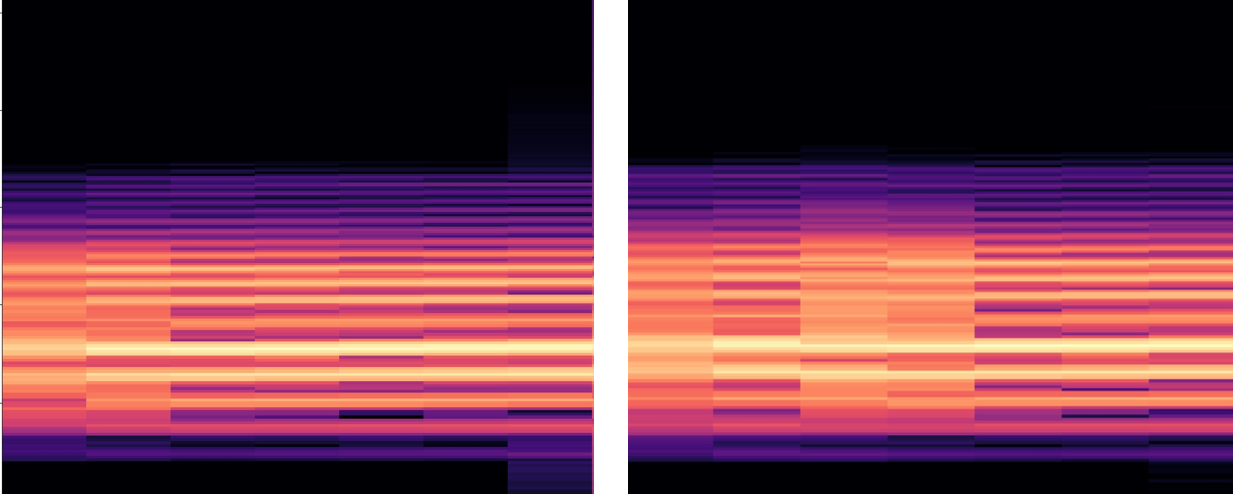
\includegraphics[width=\linewidth]{./img/augmentation/rolled}
        \caption{Przesunięcie w czasie}
        \label{fig:roll}
    \end{subfigure}

    \begin{subfigure}{0.7\textwidth}
        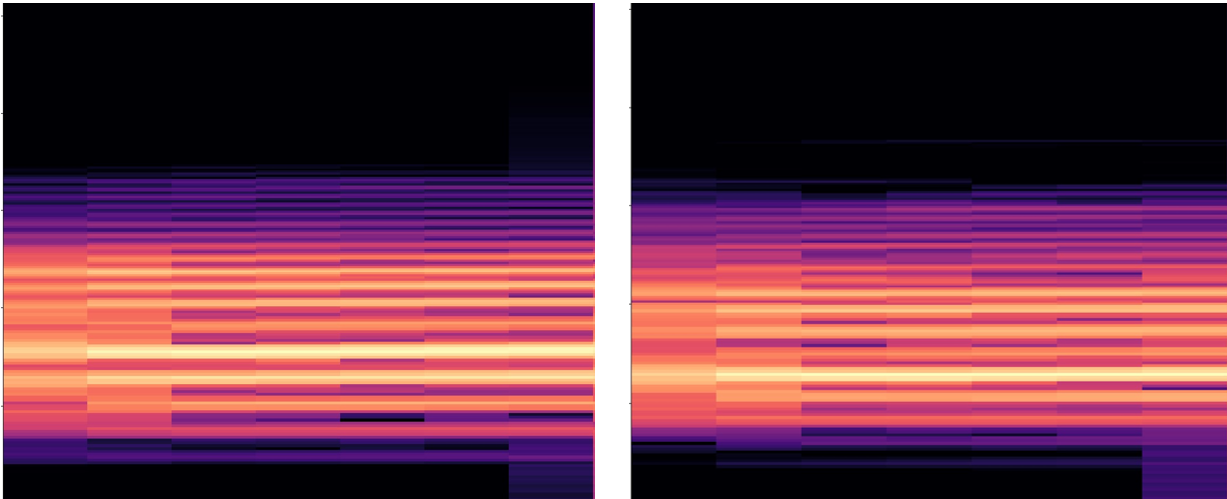
\includegraphics[width=\linewidth]{./img/augmentation/pitch}
        \caption{Zmiana wysokości dźwięku}
        \label{fig:pitch}
    \end{subfigure}

    \begin{subfigure}{0.7\textwidth}
        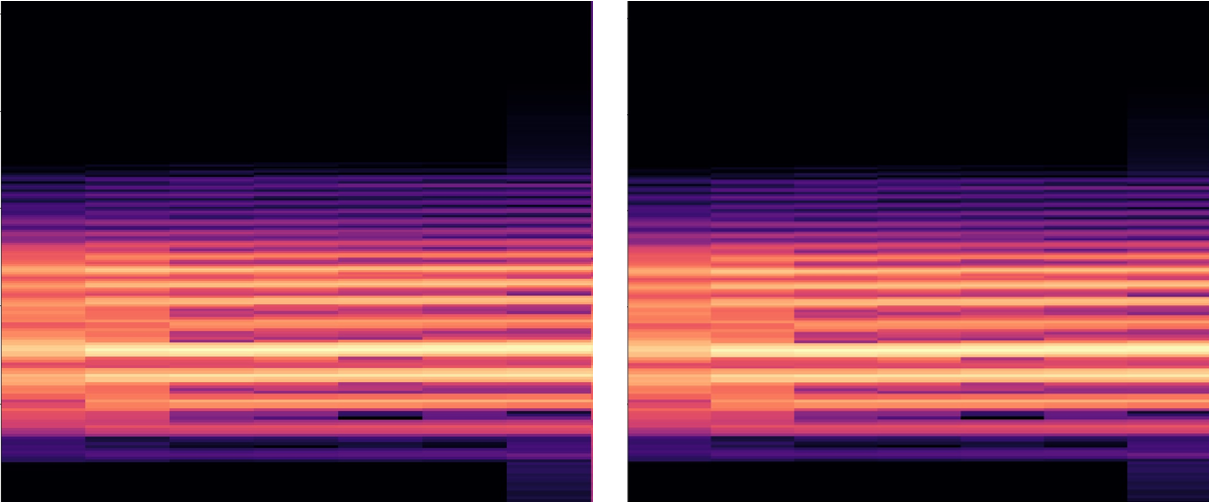
\includegraphics[width=\linewidth]{./img/augmentation/slow}
        \caption{Spowolnienie}
        \label{fig:slow}
    \end{subfigure}

    \begin{subfigure}{0.7\textwidth}
        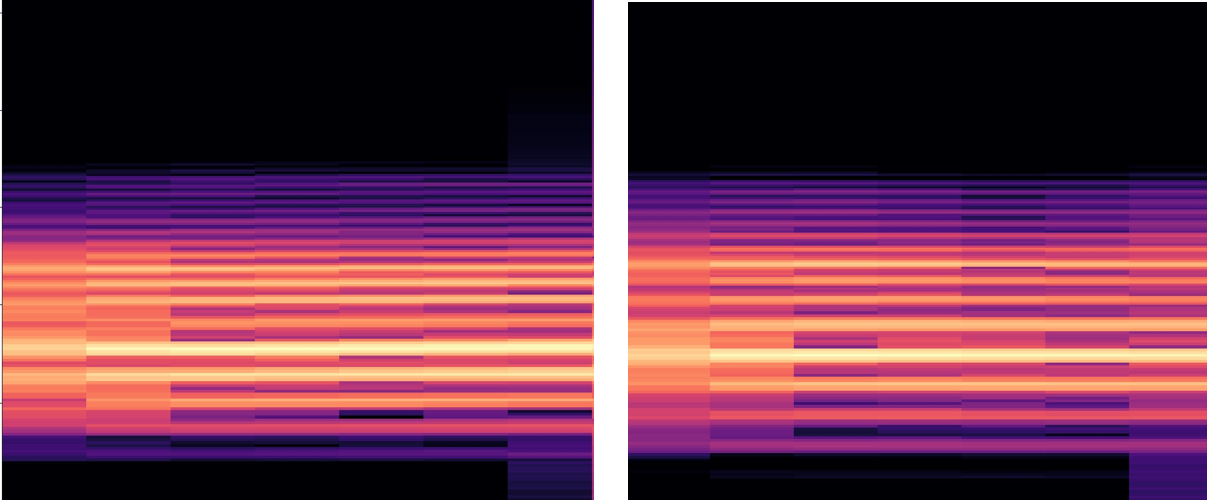
\includegraphics[width=\linewidth]{./img/augmentation/speed}
        \caption{Przyspieszenie}
        \label{fig:speed}
    \end{subfigure}

    \caption{Porównanie różnych technik augmentacji i ich wpływu na wygląd spektrogramu (zbiór danych PC-GITA, samogłoska /a/, HC)}
    \label{fig:augumentacja}
\end{figure}

%---------------------------------------------------------------------------

\section{Metody klasyfikacji}
\label{sec:klasyfikacja}

Ze względu na ograniczoną dostępność danych głosowych pacjentów z chorobą Parkinsona, zastosowano technikę znana jako \emph{transfer learning}.
Transfer learning umożliwia wykorzystanie wstępnie wytrenowanych modeli, które zostały nauczane na dużym zbiorze danych, takim jak ImageNet,
do zadań diagnostycznych z wykorzystaniem ograniczonej ilości dostępnych danych głosowych.

Kluczowym krokiem w transfer learningu było wybranie modeli, które miały dostępne wagi wytrenowane na zbiorze ImageNet.
Wybór tych modeli, takich jak Xception, MobileNetV2, Inceptionv3, VGG16 i ResNet50, był uzasadniony dostępnością wstępnie wytrenowanych wag, które zawierały ogólne cechy obrazów.
To pozwoliło na zaoszczędzenie czasu i zasobów, które byłyby potrzebne do wytrenowania sieci od podstaw na niewielkim zbiorze danych.

W ramach pracy magisterskiej skoncentrowano się na porównaniu różnych architektur klasyfikatorów w kontekście automatycznej diagnostyki choroby Parkinsona na podstawie analizy głosu.

\begin{enumerate}[label={\alph*)}]
	\item Xception
    \item [] Jest to model głębokiej nauki opracowany przez François Chollet w 2016 roku.
    Jest to jedna z odmian architektury konwolucyjnej sieci neuronowej (CNN), która wyróżnia się wyjątkową zdolnością do wykrywania cech hierarchicznych w obrazach.
    W kontekście diagnostyki choroby Parkinsona na podstawie głosu, Xception może pomóc w wyodrębnianiu istotnych cech z obrazów spektrogramów głosowych.

    \item MobileNetV2
    \item [] Jest to przykłąd lekkiej i efektywnej architektury CNN, zaprojektowanej z myślą o urządzeniach mobilnych
    Jej cechą charakterystyczną jest niska ilość parametrów i małe obliczenia, co sprawia, że jest idealna do zastosowań w zasobochłonnych zadaniach takich jak analiza głosu na urządzeniach mobilnych.

    \item InceptionV3
    \item []  Charakteryzuje się wykorzystaniem tzw. \emph{inception modules}, które pozwalają na efektywne wykrywanie wielu skal i rodzajów cech w obrazach.
    To sprawia, że Inceptionv3 może być przydatny w diagnostyce choroby Parkinsona, gdzie istotne mogą być różne aspekty głosu.
    Został zaprojektowany przez Google.

    \item VGG16
    \item [] To przykład klasycznego modelu CNN o głębokiej architekturze, opracowany przez Visual Geometry Group na Uniwersytecie Oksfordzkim.
    Jest znany ze swojej prostoty i skuteczności w ekstrakcji cech z obrazów.
    Pomimo swojej głębokości, może być użyteczny w diagnostyce na podstawie głosu, szczególnie jeśli głosowe dane wejściowe są w formie spektrogramów.

    \item ResNet50
    \item [] Jest to znana architektura CNN, która wprowadza innowacyjny pomysł na połączenia pomostowe, eliminujące problem znikającego gradientu w głębokich sieciach.
    Dzięki temu ResNet50 jest w stanie efektywnie uczyć się reprezentacji danych.
    W diagnostyce na podstawie głosu może pomóc w wykrywaniu subtelnych cech charakterystycznych dla choroby Parkinsona.
\end{enumerate}

Wybór tych konkretnych klasyfikatorów wynikał z różnorodności ich architektur i specjalizacji.
Choroba Parkinsona manifestuje się na różne sposoby w głosie pacjentów, dlatego zróżnicowane modele w różny sposób mogą wspomagać wydobycie istotnych cech.

Xception i Inceptionv3 są znane z efektywności w ekstrakcji wielu rodzajów cech, co jest istotne przy analizie złożonych danych głosowych.
MobileNetV2, z kolei, jest lekki i mobilny, co pozwala na przenośność rozwiązania do urządzeń mobilnych, które mogą być używane w codziennym monitoringu pacjentów.
VGG16 i ResNet50, choć głębokie, mają zdolność do wyodrębniania skomplikowanych wzorców, co może być przydatne w diagnozie.

Wybór tych różnorodnych klasyfikatorów pozwoli na rzetelne porównanie ich wydajności i skuteczności w diagnostyce na podstawie głosu, co może przyczynić się do lepszego zrozumienia, który model najlepiej radzi sobie z tym zadaniem.

Po wstępnym treningu na ImageNet, przeprowadzono proces fine-tuningu na zbiorze danych zawierającym nagrania głosowe pacjentów związane z diagnozą choroby Parkinsona.
Fine-tuning jest kluczowym etapem w procesie dostosowywania wstępnie wytrenowanych klasyfikatorów do konkretnej diagnozy na podstawie głosu.
W trakcie fine-tuningu modele były dostosowywane, aby nauczyć się rozpoznawania specyficznych cech akustycznych charakterystycznych dla pacjentów z chorobą Parkinsona.

Proces fine-tuningu umożliwiał dostosowanie wag i parametrów modeli do konkretnego zadania diagnostycznego, co znacząco wpłynęło na ich zdolność do rozpoznawania cezur w głosie pacjentów z tą chorobą.
W ten sposób klasyfikatory stały się bardziej odpowiednie do analizy dźwięku i diagnozy choroby Parkinsona na podstawie danych głosowych.

Wykorzystanie wstępnego treningu na ImageNet i fine-tuningu pozwoliło na połączenie ogólnych cech wyuczone przez modele w trakcie wstępnego treningu z cechami charakterystycznymi dla danych głosowych pacjentów z chorobą Parkinsona, co przyczyniło się do poprawy skuteczności diagnostyki opartej na głosie.
%---------------------------------------------------------------------------

\section{Metody ewaluacji wyników}
\label{sec:metody-ewaluacji-wynikow}

W celu oceny skuteczności różnych metod klasyfikacji choroby Parkinsona, przeprowadzono badania wykorzystujące różnorodne techniki ewaluacji.
Niniejsza sekcja zawiera prezentację wybranych metod, które zostały użyte w ramach przeprowadzonych eksperymentów.
Kluczowym aspektem tych eksperymentów jest konieczność zastosowania odpowiednich technik walidacji wyników.
Techniki te nie tylko umożliwiają obiektywną ocenę efektywności proponowanych rozwiązań, ale także pozwalają na porównanie ich ze sobą.
Dzięki temu pozwalają lepiej zrozumieć, które podejścia są najbardziej obiecujące w kontekście diagnozowania choroby Parkinsona i polepszania dokładności klasyfikacji, co jest kluczowe dla postępu w dziedzinie medycyny i diagnostyki tej choroby.

\subsection{Krzywe uczenia}
\label{subsec:krzywe-uczenia}

Krzywe uczenia są skutecznym narzędziem do wizualizacji procesu uczenia modelu.
W trakcie eksperymentów prowadzono monitorowanie dwóch kluczowych krzywych: dokładność (ang. \emph{accuracy}) i funkcję kosztu (ang. \emph{loss}).
Krzywa dokładności przedstawia zmiany dokładności modelu w trakcie treningu i walidacji, podczas gdy krzywa funkcji kosztu pokazuje, jak zmienia się funkcja kosztu w trakcie uczenia.
Analiza tych krzywych dostarcza istotnych informacji na temat efektywności uczenia modelu. Pozwala ocenić, czy model uczy się poprawnie, czy może występują problemy z
nadmiernym dopasowaniem  (ang. \emph{overfitting}) lub niedostatecznym dopasowaniem (ang. \emph{underfitting}).
Dzięki tym analizom można dokonać wniosków na temat jakości modelu i ewentualnie dostosować hiperparametry lub strategię treningową w celu uzyskania lepszych wyników.
Wartościowe informacje o procesie uczenia są kluczowe dla udanej implementacji modelu i oceny jego skuteczności.

\subsection{Metryki walidacyjne}
\label{subsec:metryki-waldiacyjne}

Podczas oceny skuteczności klasyfikacji, korzystano z najbardziej popularnych metryk, które pozwalają ocenić jakość predykcji modelu.
W podanych wzorach zastosowano oznaczenia:  TP – True Positive, TN – True Negative, FP – False Positive, FN – False Negative.

\begin{enumerate}[label={\alph*)}]
	\item Dokładność (ang.~\emph{accuracy})
    \item [] To prosta i intuicyjna miara, która oblicza stosunek poprawnie sklasyfikowanych próbek do wszystkich próbek.
    Wyraża ona ogólną skuteczność klasyfikacji.
    Wyrażana jest wzorem \ref{eq:accuracy}
    \begin{equation}
        \frac{TP + TN}{TP + FN + TN + FP}\label{eq:accuracy}
    \end{equation}
    \item Precyzja (ang.~\emph{precision})
    \item [] Mierzy stosunek prawdziwie pozytywnych predykcji do sumy prawdziwie pozytywnych i  fałszywie pozytywnych predykcji.
Wyraża zdolność modelu do identyfikowania prawdziwie pozytywnych przypadków.
Określa się ją wzorem \ref{eq:precision}
      \begin{equation}
        \frac{TP}{TP + FP}\label{eq:precision}
    \end{equation}
    \item Czułość (ang.~\emph{recall})
    \item [] Jest to stosunek prawdziwie pozytywnych predykcji do sumy prawdziwie pozytywnych i fałszywie negatywnych predykcji. Wyrażana jest wzorem \ref{eq:recall} i określa zdolność modelu do wykrywania wszystkich prawdziwie pozytywnych przypadków.
    \begin{equation}
        \frac{TP}{TP + FN}\label{eq:recall}
    \end{equation}
    \item Miara F1 (ang.~\emph{F1-score})
    \item [] To harmoniczna średnia precyzji i czułości. Jest używana jako miara równowagi między precyzją a czułością. Wyższe wartości wskazują na lepszą jakość klasyfikacji modelu. Wyraża się ją wzorem \ref{eq:f1}.
  \begin{equation}
        \frac{2 * TP}{2 * TP + FP + FN}\label{eq:f1}
    \end{equation}
\end{enumerate}


\subsection{Macierz pomyłek}
\label{subsec:macierz-pomylek}

Macierz pomyłek to narzędzie służące do analizy wyników klasyfikacji.
Przedstawia ona liczbę prawidłowo i błędnie zaklasyfikowanych próbek dla każdej klasy.
Na podstawie macierzy pomyłek możemy obliczyć błędy I i II rzędu.
\begin{enumerate}[label={\alph*)}]
	\item Błąd I rzędu (ang. \emph{False Positive}) oznacza błędną klasyfikację przypadku, który jest negatywny, jako pozytywny.
    W kontekście Parkinsona, błąd I rzędu oznacza, że model zaklasyfikował zdrową osobę jako chorą na chorobę Parkinsona.
\item Błąd II rzędu (ang. \emph{False Negative}) oznacza błędną klasyfikację przypadku, który jest pozytywny, jako negatywny.
    W kontekście Parkinsona, błąd II rzędu oznacza, że model zaklasyfikował osobę chorą na chorobę Parkinsona jako zdrową.
\end{enumerate}

Analiza błędów I i II rzędu ma duże znaczenie w kontekście ewaluacji systemów diagnostycznych.
Błąd I rzędu może prowadzić do niezdiagnozowania choroby u pacjenta, podczas gdy błąd II rzędu może prowadzić do błędnego zdiagnozowania osoby zdrowej jako cierpiącej na chorobę Parkinsona.
Ważne jest, aby oceniać i minimalizować te błędy w celu uzyskania jak najdokładniejszej klasyfikacji.